\documentclass{estilos/tesisuchile2-espaniol}

% Portada - Variables
\facultad{NOMBRE DE LA FACULTAD} 
\departamento{NOMBRE DEL DEPARTAMENTO}
\titulo{Plantilla de Tesis en Espa\~nol v\version}
\subtitulo{De acuerdo a las normas de la Universidad de Chile para escribir en espa\~nol}
\trabajoygrado{Tesis para optar al grado de INSERTAR GRADO}

\autoruno{ALUMNO}
%\mailautoruno{mauriciovargas@ug.uchile.cl}
%\autordos{poner autor dos}
%\mailautordos{poner mail autor dos}

\profguia{NOMBRE DEL PROF. GUIA} %profesor guia
\profintuno{PROF. INTEGRANTE 1} %profesor integrante 1
\profintdos{PROF. INTEGRANTE 2} %profesor integrante 2, se puede borrar esta linea
\profinttres{PROF. INTEGRANTE 3} %profesor integrante 2, se puede borrar esta linea
%\proyecto{Financiado por el proyecto \#ZZZZ} %lponer proyecto y financiamiento, se puede borrar esta linea 

\ciudad{CIUDAD} \pais{PAIS} \monthpub{MES} \yearpub{A\~NO}

\begin{document}

%% Portada
\maketitle

%lista de tareas pendientes (usar \pacha{}, etc)
\thispagestyle{empty}
\hbox{}
\cleardoublepage
\listoftodos

% Prefacio
\thispagestyle{empty}
\hbox{}
\cleardoublepage

\begin{preface}

\section{Resumen}

Este es un texto\edgar{comentario de ejemplo 1}\: de\pacha{comentario de ejemplo 2}\: ejemplo:
\\Lorem ipsum dolor sit amet, consectetur adipiscing elit, sed do eiusmod tempor incididunt ut labore et dolore magna aliqua. Ut enim ad minim veniam, quis nostrud exercitation ullamco laboris nisi ut aliquip ex ea commodo consequat. Duis aute irure dolor in reprehenderit in voluptate velit esse cillum dolore eu fugiat nulla pariatur. Excepteur sint occaecat cupidatat non proident, sunt in culpa qui officia deserunt mollit anim id est laborum.

\bigskip

\bigskip

Palabras clave: \emph{INSERTAR PALABRAS CLAVE}.

% Pagina Optativa - Dedicatoria

\cleardoublepage
\thispagestyle{empty}
\hbox{ }
\cleardoublepage

\section{Dedicatoria}

\begin{center}
\emph{Dedicado a \ldots INSERTAR DEDICATORIA \ldots}
\end{center}

\cleardoublepage
\thispagestyle{empty}
\hbox{ }
\cleardoublepage

% Pagina Optativa - Agradecimientos
\section{Agradecimientos}

A las personas que aportaron\ldots INSERTAR AGRADECIMIENTOS \ldots

% Indice - General
\cleardoublepage
\thispagestyle{empty}
\hbox{ }
\cleardoublepage

\tableofcontents

% Indice - Tablas
\cleardoublepage
\thispagestyle{empty}
\hbox{ }
\cleardoublepage

\listoftables

% Indice - Figuras
\cleardoublepage
\thispagestyle{empty}
\hbox{ }
\cleardoublepage

\listoffigures

\end{preface}

% Introduccion
\chapter{NOMBRE DEL CAPITULO 1}\label{cap1}

\begin{flushright}
INSERTAR CITA RELEVANTE (OPCIONAL)
\end{flushright}
 
\section{SECCION 1}

Por completitud incluyo una cita en Bibtex: \citep{bock2010stats}.

Texto de ejemplo: Sed ut perspiciatis unde omnis iste natus error sit voluptatem accusantium doloremque laudantium, totam rem aperiam, eaque ipsa quae ab illo inventore veritatis et quasi architecto beatae vitae dicta sunt explicabo. Nemo enim ipsam voluptatem quia voluptas sit aspernatur aut odit aut fugit, sed quia consequuntur magni dolores eos qui ratione voluptatem sequi nesciunt. Neque porro quisquam est, qui dolorem ipsum quia dolor sit amet, consectetur, adipisci velit, sed quia non numquam eius modi tempora incidunt ut labore et dolore magnam aliquam quaerat voluptatem. Ut enim ad minima veniam, quis nostrum exercitationem ullam corporis suscipit laboriosam, nisi ut aliquid ex ea commodi consequatur? Quis autem vel eum iure reprehenderit qui in ea voluptate velit esse quam nihil molestiae consequatur, vel illum qui dolorem eum fugiat quo voluptas nulla pariatur?

\subsection{SUB-SECCION 1}

Texto de ejemplo: At vero eos et accusamus et iusto odio dignissimos ducimus qui blanditiis praesentium voluptatum deleniti atque corrupti quos dolores et quas molestias excepturi sint occaecati cupiditate non provident, similique sunt in culpa qui officia deserunt mollitia animi, id est laborum et dolorum fuga. Et harum quidem rerum facilis est et expedita distinctio. Nam libero tempore, cum soluta nobis est eligendi optio cumque nihil impedit quo minus id quod maxime placeat facere possimus, omnis voluptas assumenda est, omnis dolor repellendus. Temporibus autem quibusdam et aut officiis debitis aut rerum necessitatibus saepe eveniet ut et voluptates repudiandae sint et molestiae non recusandae. Itaque earum rerum hic tenetur a sapiente delectus, ut aut reiciendis voluptatibus maiores alias consequatur aut perferendis doloribus asperiores repellat. 
\cleardoublepage
\thispagestyle{empty}
\hbox{ }
\cleardoublepage

\chapter{NOMBRE DEL CAPITULO 2}\label{cap2}

\begin{flushright}
INSERTAR CITA RELEVANTE (OPCIONAL)
\end{flushright}
 
\section{SECCION 1: ALGUNAS ECUACIONES}

\subsection{Serie geom\'etrica}

Sea $r\in (0,1)$ se tiene que la suma de exponentes consecutivos de $r^i$ converge, es decir
\begin{equation}
\sum_{i=0}^{\infty} r^i = \frac{1}{1-r}
\end{equation}
notamos que $r$ puede crecer de manera tal que
$$
\lim_{r\to \infty} \frac{1}{1-r} = 0
$$
o escrito de otra manera
$$
\sum_{i=0}^{\infty} r^i = \frac{1}{1-r} \stackrel{r\to \infty}{\longrightarrow} 0
$$

\subsection{Distribuci\'on Normal}

\begin{equation}
\mathcal{N}(\mu,\sigma^2) = \int\limits_{-\infty}^{x} \frac1{\sigma\sqrt{2\pi}}\: \exp{-\frac{1}{2}\left(\frac{t-\mu}{\sigma}\right)^2}\: dt
\end{equation} 

% Apendices
\cleardoublepage
\thispagestyle{empty}
\hbox{ }
\cleardoublepage

\appendix 

\section{INSERTANDO IMAGENES, TABLAS, CODIGO, ETC}

Im\'agenes:
\begin{figure}[h]
\centering
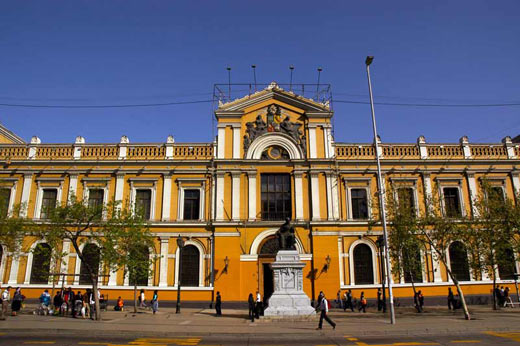
\includegraphics[scale=0.8]{figuras/uchile.jpg} 
\caption{\textsf{Universidad de Chile (escala 80\%)}}
\end{figure}

C\'odigo C, R, Java, etc:
\lstinputlisting{codigo/cargar-librerias.R}

\newpage

Tabla:

\begin{table}[h]
\centering
\begin{tabular}{l*{6}{c}r}
Variable              & Obs 1 & Obs 2 & Obs 3 & Obs 4 & Obs 5\\
\hline
V1 & 6 & 4 & 0 & 2 & 10 \\
V2            & 6 & 3 & 0 & 3 &  8 \\
V3           & 6 & 2 & 1 & 3 &  7 \\
V4     & 6 & 2 & 1 & 3 &  5 \\
\end{tabular}
    \caption{Tabla de ejemplo.}
\end{table}

% Bibliografia
\cleardoublepage
\addcontentsline{toc}{chapter}{Bibliograf\'ia}
\printbibliography

\end{document}